% =====================================================================
% Anexo G: resultados complementarios (adaptacion de Sonata, variantes de
% fusion, una sola semilla y sensibilidad a K).
% =====================================================================

\section*{Anexo G. Resultados complementarios}
\label{sec:anexo-complementarios}
\phantomsection\addcontentsline{toc}{section}{Anexo G. Resultados complementarios}

\setcounter{figure}{0}\renewcommand{\thefigure}{G.\arabic{figure}}
\setcounter{table}{0}\renewcommand{\thetable}{G.\arabic{table}}

Este anexo reúne los resultados que sustentan lo dicho en la
Sección~\ref{sec:res-unidad3} pero que no hacen falta para seguir su argumento.

\subsection*{G.1. Adaptación de Sonata a la Catedral}

Se continuó el preentrenamiento auto-supervisado de Sonata con 21 escaneos de la
Catedral, sin etiquetas y sin PL7 ni PL13, que se dejaron fuera para evaluar. El
entrenamiento, de 30 épocas y 3\,150 iteraciones con lote 1, tardó 103\,min en una
GPU L4. Se usó el \emph{teacher} de la época 30. La Tabla~\ref{tab:g-sonata}
compara el descriptor original con el adaptado sobre PL13 y la
Figura~\ref{fig:g-sonata-m3} lo muestra. El descriptor adaptado se parece al
original solo en parte, con un coseno medio de 0{,}54, es menos estable al
agrupar con $K=8$ y tiene menos dimensiones efectivas. Con etiquetas, sin
embargo, empeora a M3 (Tabla~\ref{tab:m2-m4-semillas}), de modo que no se
adoptó.

\begin{table}[!htbp]
\centering
\setstretch{1}\small
\caption[Sonata original y adaptado sobre PL13]{Descriptor $f_{\mathrm{ssl}}$ original y adaptado sobre PL13, sin etiquetas. Elaboración propia a partir de los registros del experimento de adaptación.}
\label{tab:g-sonata}
\begin{tabular}{@{}lrr@{}}
\toprule
\textbf{Medida} & \textbf{Original} & \textbf{Adaptado} \\
\midrule
Coseno medio entre ambos descriptores & \multicolumn{2}{c}{0,543} \\
ARI entre ambos agrupamientos, $K=8$ & \multicolumn{2}{c}{0,211} \\
Rango efectivo & 110,5 & 81,3 \\
Estabilidad del $k$-means, $K=8$ (ARI) & 0,610 & 0,492 \\
Varianza de las 3 primeras componentes & 0,253 & 0,225 \\
Extracción en PL13 & 13,9\,s, 34,60\,GB (A6000) & 20,3\,s, 7,40\,GB (L4) \\
\bottomrule
\end{tabular}
\end{table}

La memoria de la última fila no es comparable entre columnas: el equipo es
distinto y el adaptado se extrajo con la atención \texttt{SDPA} de PyTorch, que
usa mucha menos memoria que la atención densa del original.

\begin{figure}[!htbp]
\centering
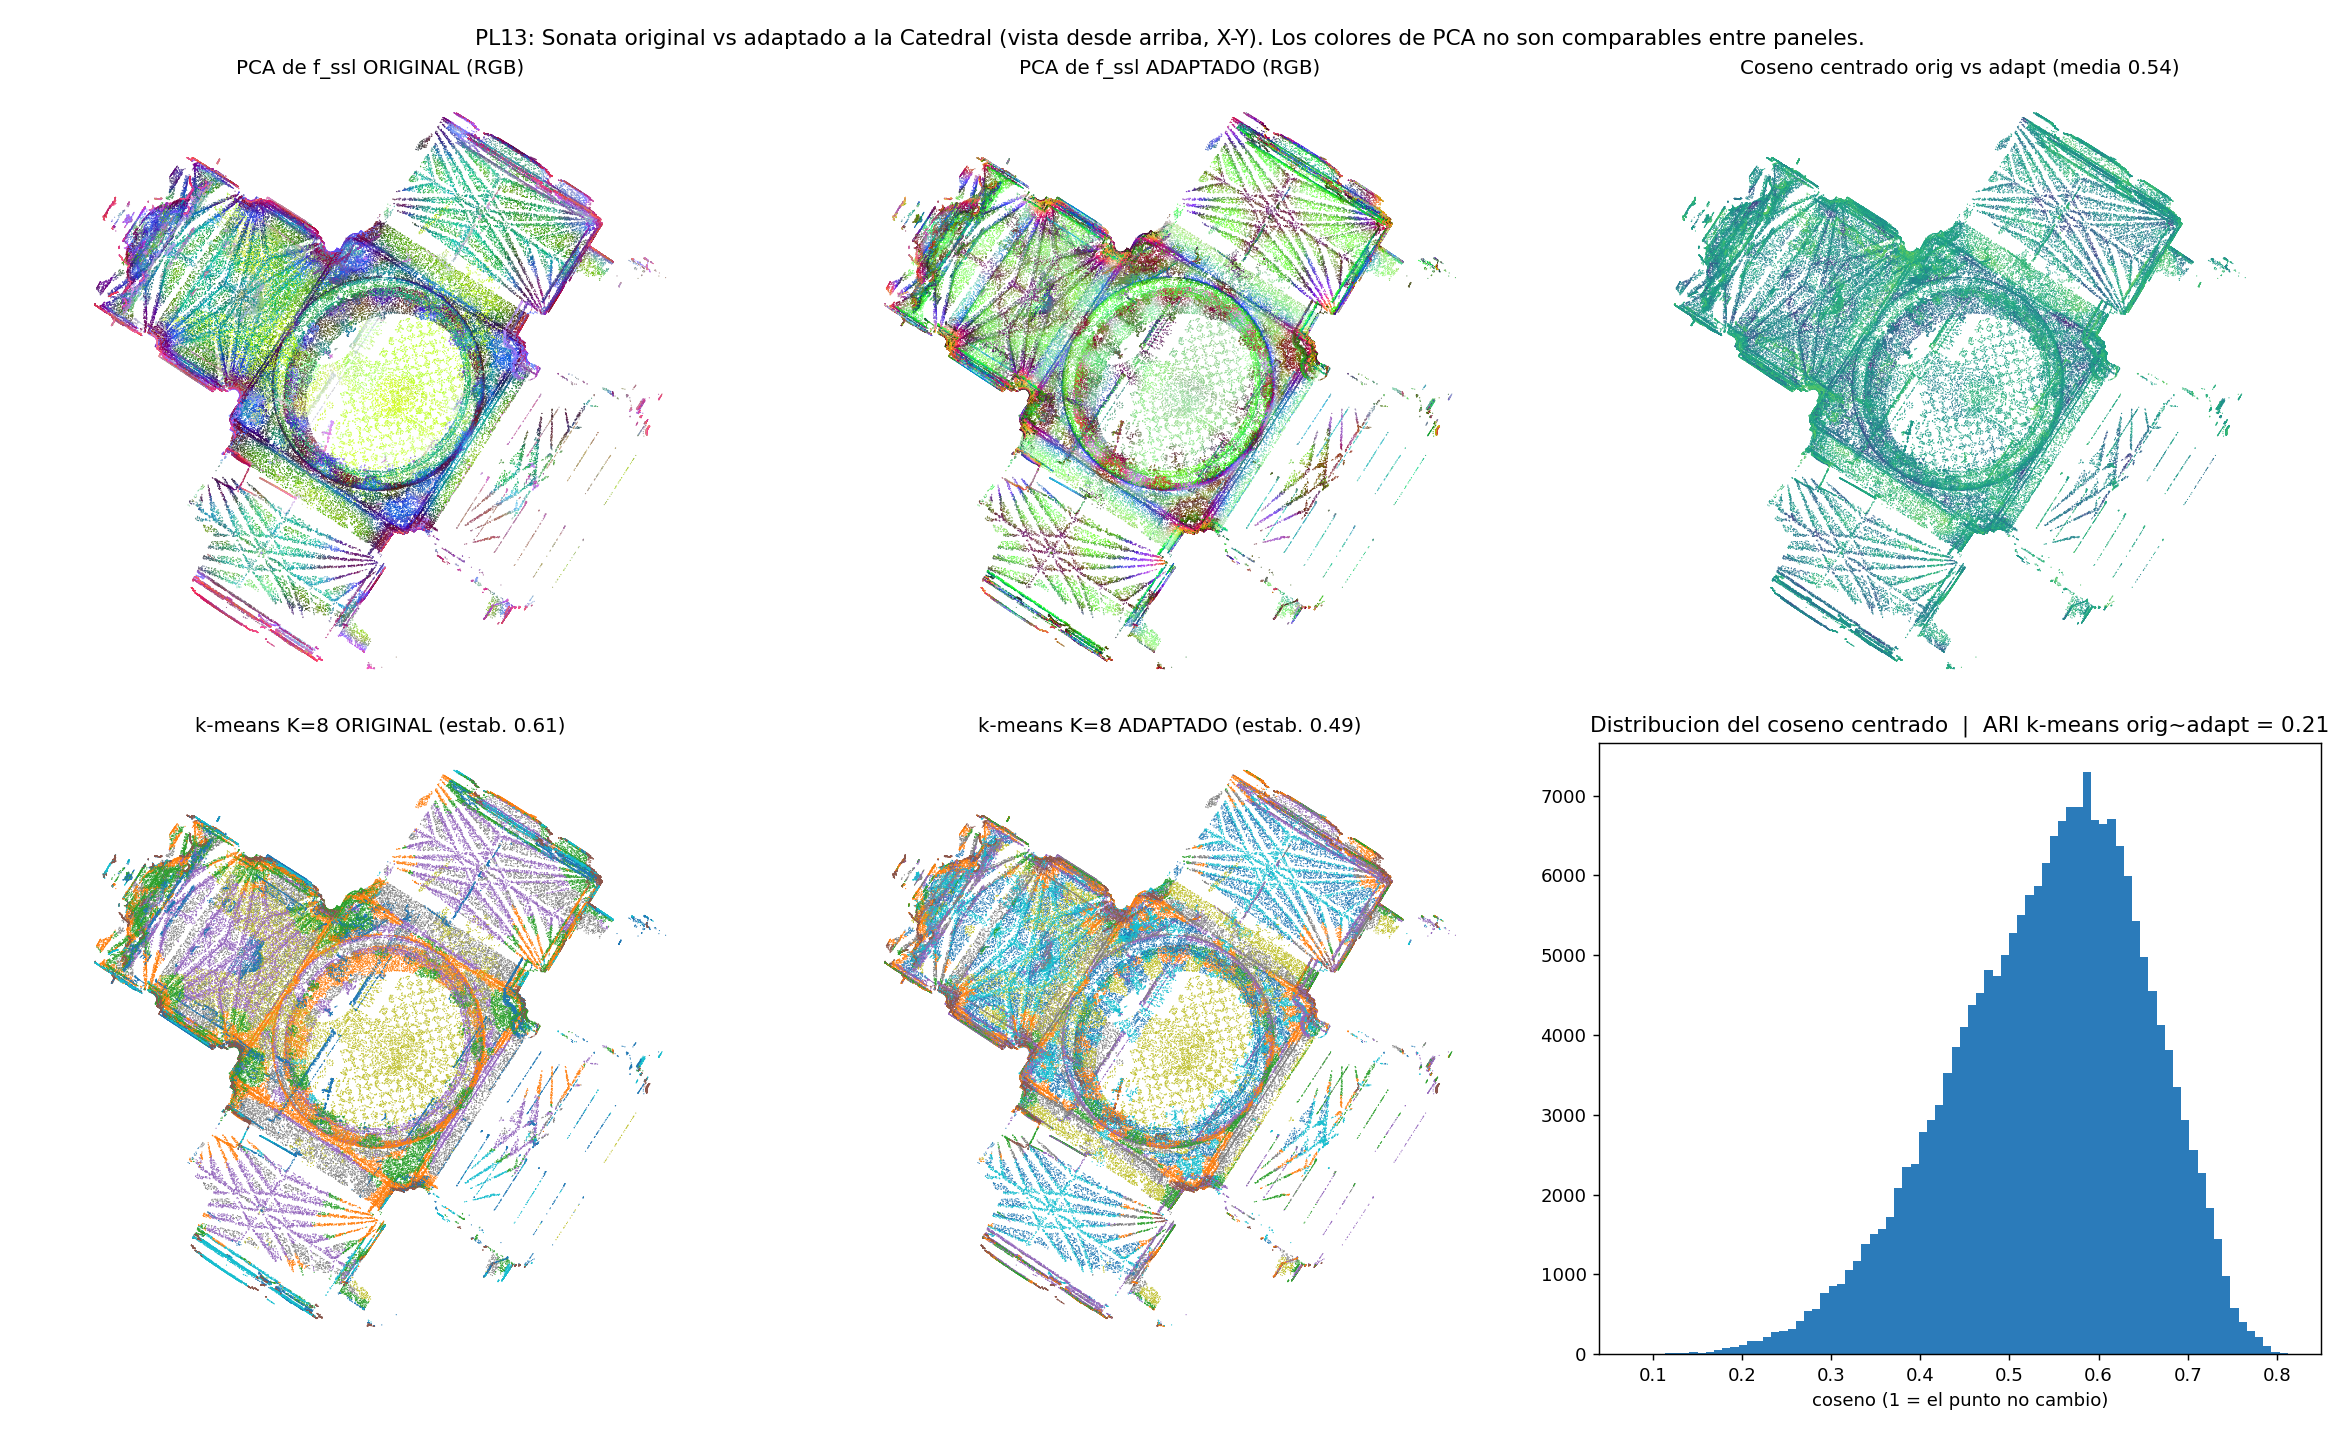
\includegraphics[width=\linewidth]{imagenes/sonata_adaptado_m3.png}
\caption[Sonata original y adaptado sobre PL13]{Comparación del descriptor de
Sonata original y adaptado sobre PL13: similitud por coseno, componentes
principales y $k$-means. Elaboración propia.}
\label{fig:g-sonata-m3}
\end{figure}

\begin{figure}[!htbp]
\centering
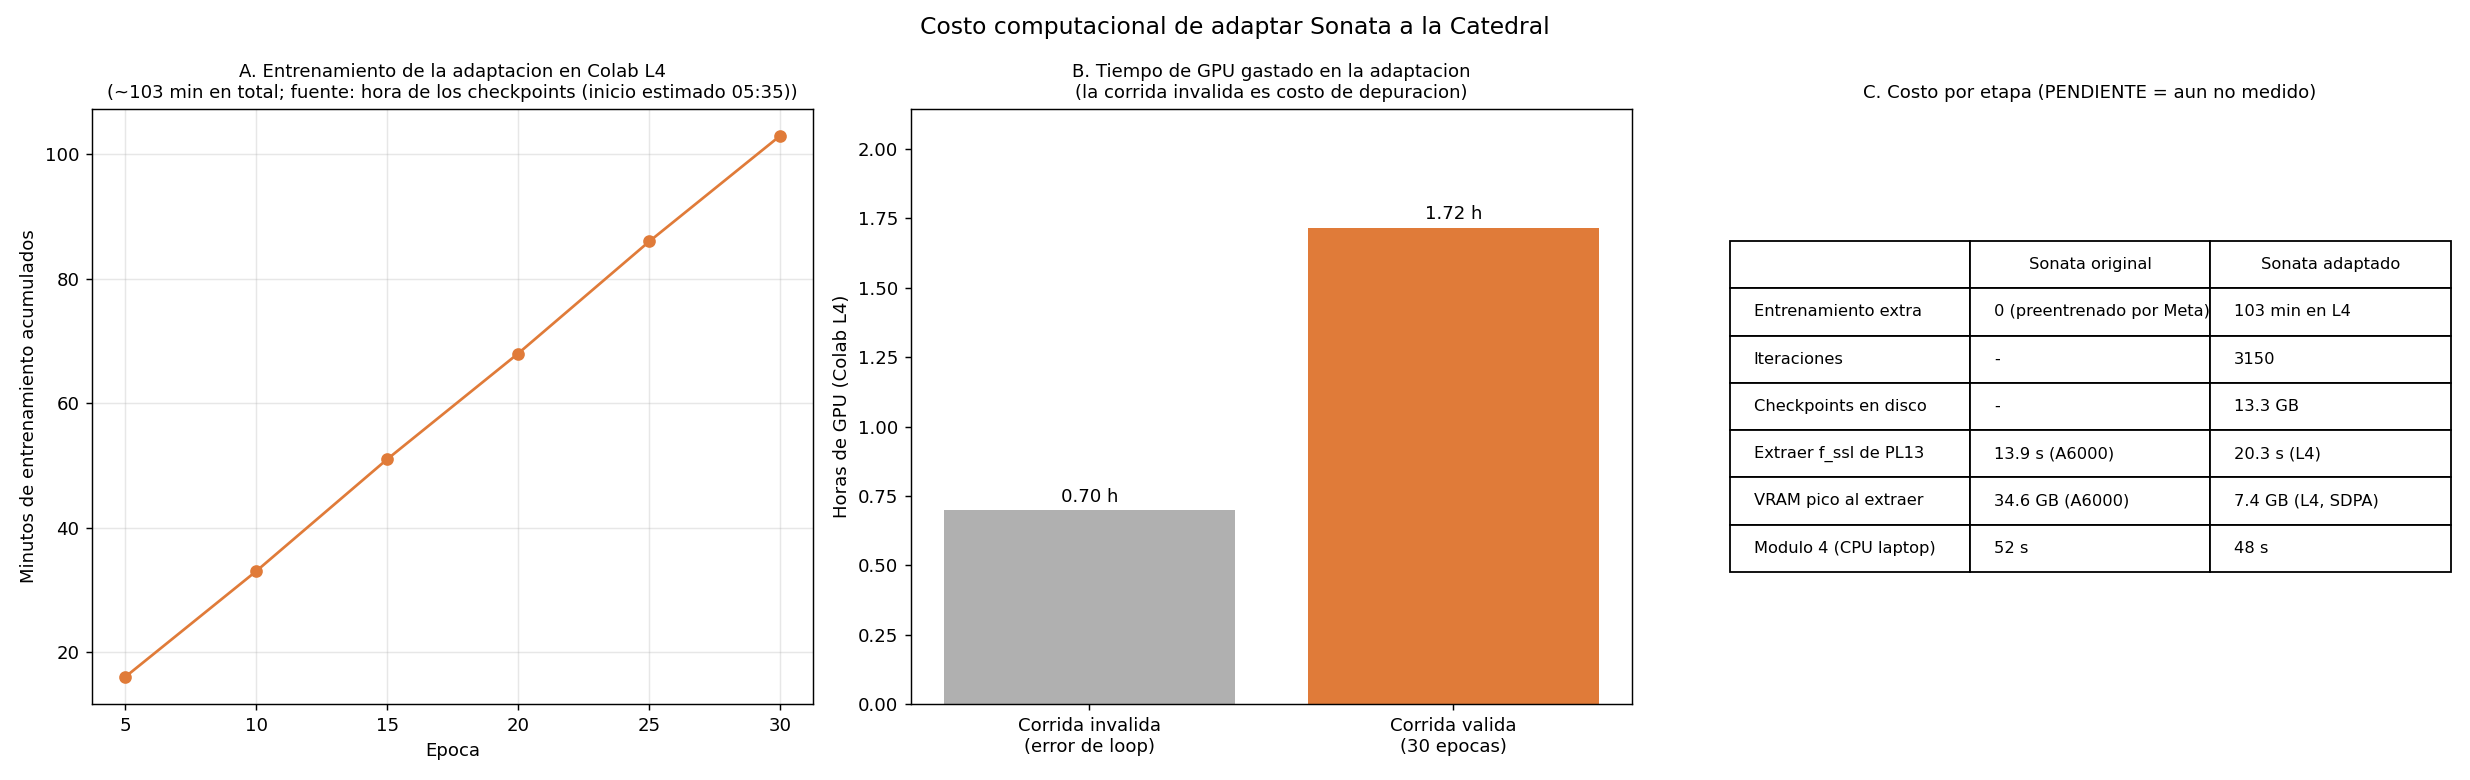
\includegraphics[width=0.85\linewidth]{imagenes/sonata_costo.png}
\caption[Costo computacional de adaptar Sonata]{Costo computacional de adaptar
Sonata a la Catedral y de extraer sus descriptores. Elaboración propia.}
\label{fig:g-sonata-costo}
\end{figure}

\subsection*{G.2. Una sola semilla frente a diez}

Con una sola semilla el orden de los métodos cambia. La Tabla~\ref{tab:g-una}
muestra que M4 queda por debajo de M4 base con M2 de ArCH y Sonata original
(50,6 frente a 52,9), mientras que con diez semillas queda por encima (52,5
frente a 51,4; Tabla~\ref{tab:m2-m4-semillas}). Por eso la comparación se repite
con diez semillas y se reporta su dispersión.

\begin{table}[!htbp]
\centering
\setstretch{1}\small
\caption[mIoU con una sola semilla]{mIoU uno a uno (\%) sin \emph{other}, con $K=8$ y una sola semilla, en la capilla. Elaboración propia.}
\label{tab:g-una}
\begin{tabularx}{\linewidth}{@{}>{\raggedright\arraybackslash}Xrrrr@{}}
\toprule
\textbf{Método} & \textbf{SemanticPOSS + orig.} & \textbf{ArCH + orig.} & \textbf{SemanticPOSS + adap.} & \textbf{ArCH + adap.} \\
\midrule
M2 & 34,1 & 49,0 & 34,1 & 49,0 \\
M3 & 53,4 & 52,5 & 35,6 & 35,1 \\
M4 base & 32,1 & 52,9 & 32,1 & 52,9 \\
M4 & 52,5 & 50,6 & 36,1 & 47,4 \\
\bottomrule
\end{tabularx}
\end{table}

\subsection*{G.3. Variantes de fusión}

Se probaron fusiones deterministas distintas de la concatenación, con media de
cinco semillas, para ver si alguna gana de forma consistente
(Figura~\ref{fig:g-variantes}). Las que mejoran en las cuatro combinaciones
suben como máximo 1,8 puntos en las dos combinaciones con M2 de ArCH. La mayor
mejora en esas columnas, 3,0 puntos, es de una configuración que baja 1,3 puntos en
otra combinación. Con el M2 de SemanticPOSS, colapsado, las variantes llegan a
subir entre 10 y 14 puntos, porque hay más margen que ganar. Al elegir la variante en una mitad de las semillas y reportarla en la
otra, la mejora con M2 de ArCH y Sonata original es de $-0{,}2$ puntos y con Sonata
adaptado, de $+1{,}1$. Ninguna variante se adoptó.

\begin{figure}[!htbp]
\centering
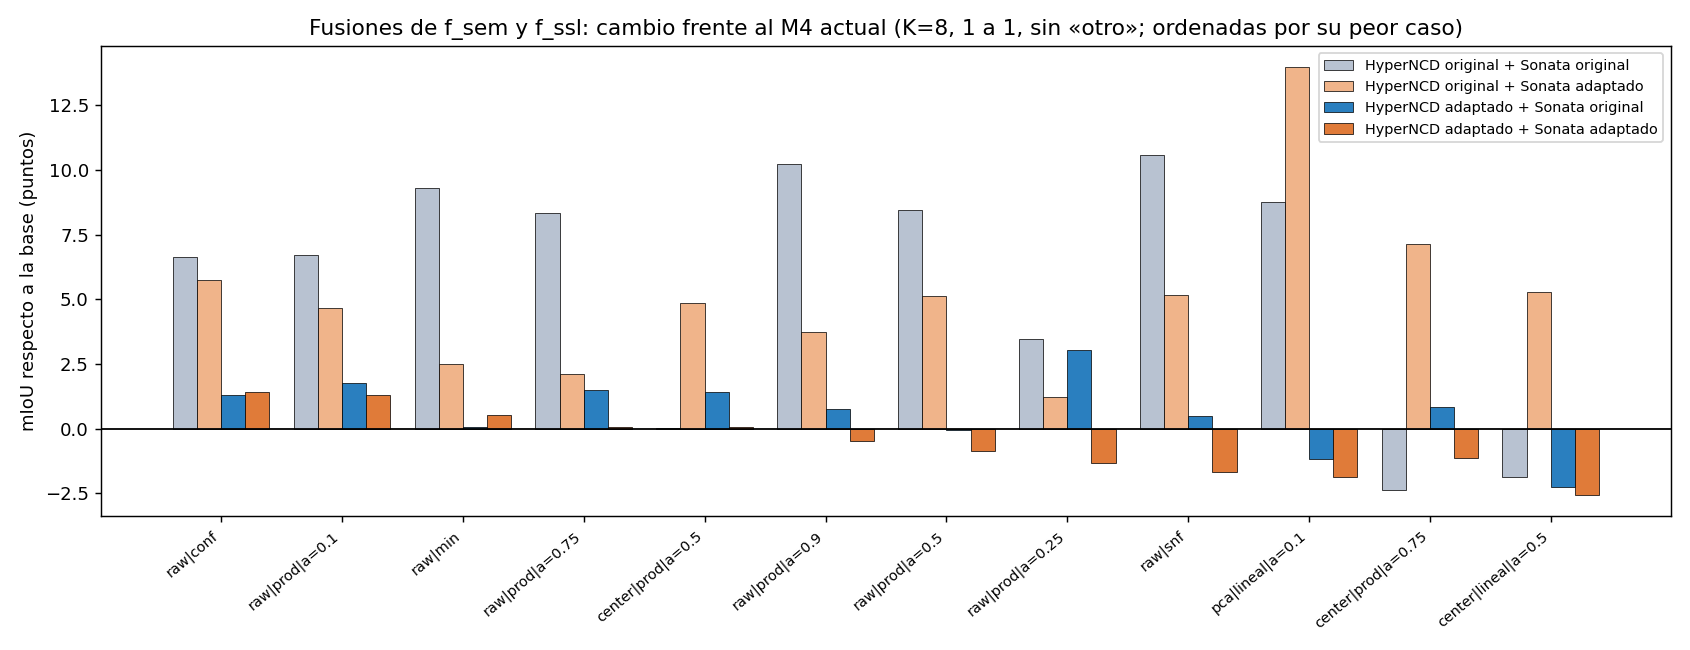
\includegraphics[width=\linewidth]{imagenes/m4_variantes_fusion.png}
\caption[Variantes de fusión de los descriptores]{Cambio de mIoU, en puntos,
de cada variante de fusión respecto del M4 actual en las cuatro combinaciones de
M2 y Sonata. Elaboración propia.}
\label{fig:g-variantes}
\end{figure}

\subsection*{G.4. Sensibilidad al número de grupos}

La Figura~\ref{fig:g-miou-k} muestra el mIoU de cada módulo para $K=6$, 8 y 12,
con y sin \emph{other}, para el M2 de ArCH con Sonata original y adaptado, con
una sola semilla.

\begin{figure}[!htbp]
\centering
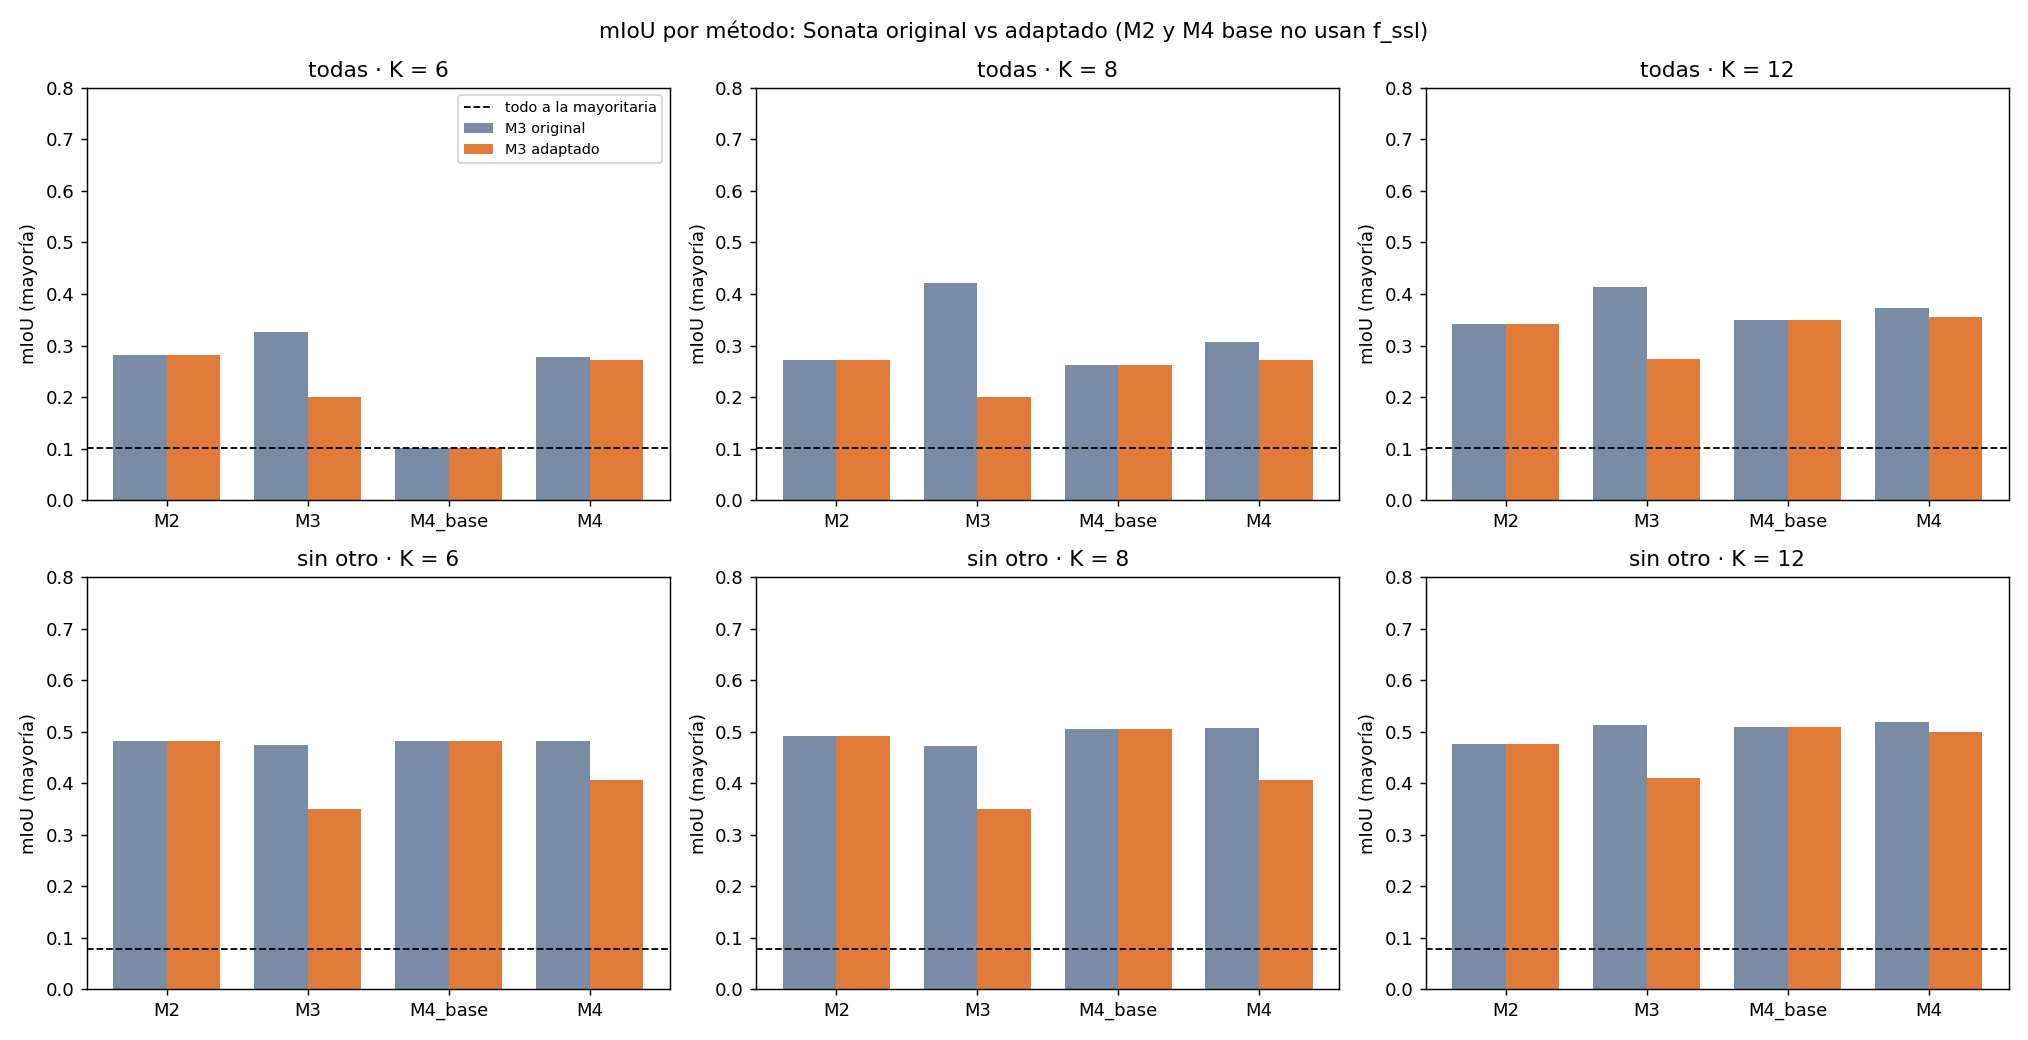
\includegraphics[width=\linewidth]{imagenes/m4_miou_por_modulo.png}
\caption[mIoU por módulo y por número de grupos]{mIoU por mayoría de M2, M3, M4
base y M4 con $K=6$, 8 y 12, con y sin \emph{other}, con Sonata original y
adaptado. Elaboración propia.}
\label{fig:g-miou-k}
\end{figure}
